\begin{frame}
  \frametitle{Nordic Mobile Telephone (NMT)}
  
  \begin{center}
    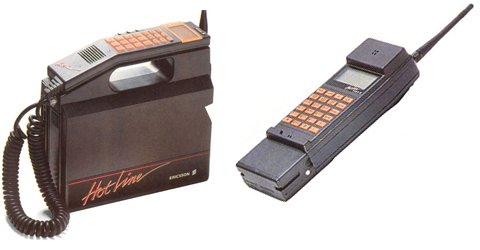
\includegraphics[width=0.55\columnwidth]{./pictures/ericsson-hotline-nmt900.jpg}
  \end{center}
\end{frame}

\begin{frame}
  \frametitle{Motivation and features}
  
    \begin{itemize}
     \item Motivation
     \begin{itemize}
      \item Overcrowding of manual mobile networks
      \item Neighboring countries used incompatible technologies
     \end{itemize}
    \end{itemize}
    
    \begin{center}
     $\Rightarrow$ Addressed by national telephone operators from\\Denmark, Finnland, Norway and Sweden
    \end{center}
    
    \begin{itemize}
     \item Results
      \begin{itemize}
	\item Same services as landline
        \item Automatized handover between calls
        \item National and international roaming
      \end{itemize}
    \end{itemize}
\end{frame}

\begin{frame}
  \frametitle{Negotiation and diffusion}
  
  \begin{chronology}[10]{1969}{1986}{3ex}{\textwidth}
    \event{1969}{Vision of a standardized system}
    \event{1970}{First meeting of operator representatives}
    %\event{1971}{System specification}
    \event[1981]{1982}{NMT-450 release (on time)}
    \event{1985}{Largest cellular phone system world-wide}
    \event{1986}{NMT-900 release}
  \end{chronology}
  
  \begin{center}
     $\Rightarrow$ NMT became a \textbf{global} standard
    \end{center}
\end{frame}

\begin{frame}
  \frametitle{Success factors}
  
  % umformulieren!
  \begin{itemize}
   \item Market orientation 
   \item Small working groups
   \item Negotiation restricted to interface specifications
   \item Intense relationship to manufacturers but neutral treatment
   \item Economies of scale due to open specification and lack of IPRs/no license fees 
   \item No/little government/national institutions involvement
  \end{itemize}
\end{frame}